\def\layersep{2.5cm}

\begin{figure}[tbp!]
    \begin{subfigure}[b]{0.49\textwidth}
        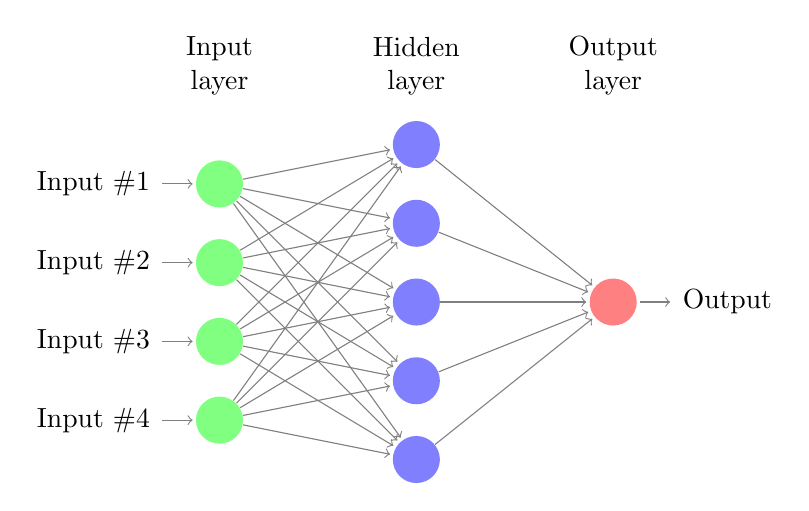
\begin{tikzpicture}[shorten >=1pt,->,draw=black!50, node distance=\layersep]
            \tikzstyle{every pin edge}=[<-,shorten <=1pt]
            \tikzstyle{neuron}=[circle,fill=black!25,minimum size=17pt,inner sep=0pt]
            \tikzstyle{input neuron}=[neuron, fill=green!50];
            \tikzstyle{output neuron}=[neuron, fill=red!50];
            \tikzstyle{hidden neuron}=[neuron, fill=blue!50];
            \tikzstyle{annot} = [text width=4em, text centered]
        
            % Draw the input layer nodes
            \foreach \name / \y in {1,...,4}
            % This is the same as writing \foreach \name / \y in {1/1,2/2,3/3,4/4}
                \node[input neuron, pin=left:Input \#\y] (I-\name) at (0,-\y) {};
        
            % Draw the hidden layer nodes
            \foreach \name / \y in {1,...,5}
                \path[yshift=0.5cm]
                    node[hidden neuron] (H-\name) at (\layersep,-\y cm) {};
        
            % Draw the output layer node
            \node[output neuron,pin={[pin edge={->}]right:Output}, right of=H-3] (O) {};
        
            % Connect every node in the input layer with every node in the
            % hidden layer.
            \foreach \source in {1,...,4}
                \foreach \dest in {1,...,5}
                    \path (I-\source) edge (H-\dest);
        
            % Connect every node in the hidden layer with the output layer
            \foreach \source in {1,...,5}
                \path (H-\source) edge (O);
        
            % Annotate the layers
            \node[annot,above of=H-1, node distance=1cm] (hl) {Hidden layer};
            \node[annot,left of=hl] {Input layer};
            \node[annot,right of=hl] {Output layer};
        \end{tikzpicture}
        \caption{}
        \label{fig: Machine learning: Perceptron}
    \end{subfigure}
    \hfill
    \begin{subfigure}[b]{0.49\textwidth}
        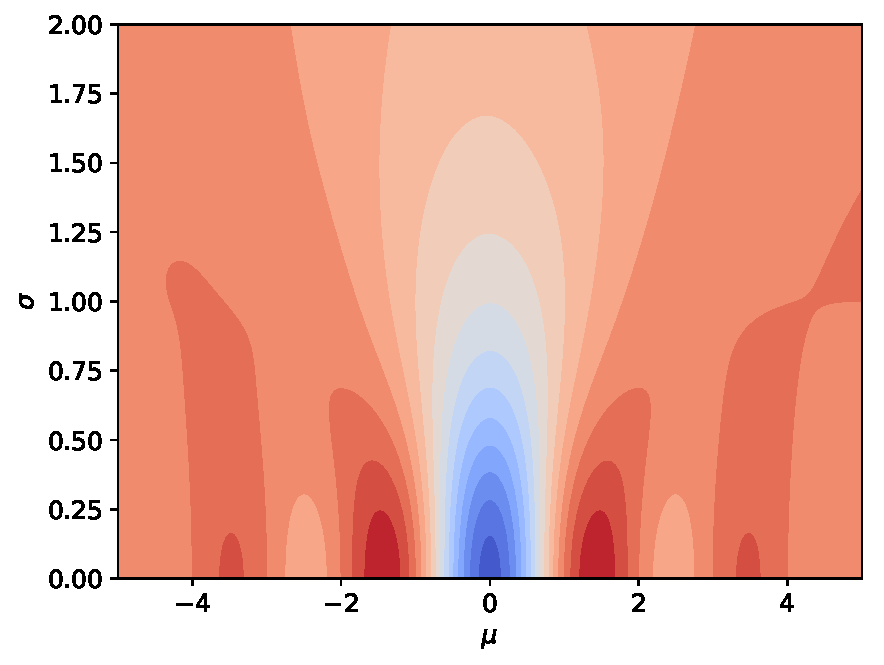
\includegraphics[width=\textwidth]{graphics/var-opt-intu/variational-optimization-contour-sinc.pdf}
        \caption{}
        \label{fig: Theory: var-opt-intu-sinc-contour}
    \end{subfigure}
    \caption{}
    \label{fig: Theory: var-opt-intu-sinc}
\end{figure}





\tikzset{%
  every neuron/.style={
    circle,
    draw,
    minimum size=.6cm
  },
  neuron missing/.style={
    draw=none, 
    scale=4,
    text height=0.333cm,
    execute at begin node={\color{black}\tiny$\vdots$}
  },
}

\begin{figure}[H]
    \centering
    \begin{tikzpicture}[x=1.5cm, y=1.5cm, >=stealth]
        % Input nodes
        \foreach \m/\l [count=\y] in {1,2,3,missing,4}
          \node [every neuron/.try, neuron \m/.try] (input-\m) at (0,2.5-\y) {};
          
        %\node [every neuron/.try, neuron \m/.try] (bias-\m) at (0,2.5-5) {};
        
        % Hidden layer nodes
        %\foreach \m [count=\y] in {1,missing,2}
        %  \node [every neuron/.try, neuron \m/.try ] (hidden-\m) at (2,2-\y*1.25) {};
        
        % Output node
        \node [every neuron/.try, neuron 1/.try ] (output-1) at (4,1.5-1) {};
        %\foreach \m [count=\y] in {1}
        %  \node [every neuron/.try, neuron \m/.try ] (output-\m) at (4,1.5-\y) {};
        
        % Names on input arrows
        \foreach \l [count=\i] in {1,2,3,I}
          \draw [<-] (input-\i) -- ++(-1,0)
            node [above, midway] {$x_\l$};
        
        %\foreach \l [count=\i] in {1,n}
        %  \node [above] at (hidden-\i.north) {$z_\l$};
        
        % Name on output arrow
        \draw [->] (output-1) -- ++(1,0)
            node [above, midway] {$y$};
        
        %\foreach \l [count=\i] in {1,n}
        %  \draw [->] (output-\i) -- ++(1,0)
        %    node [above, midway] {$y_\l$};
        
        % Inputs -> Outputs
        \foreach \i in {1,...,4}
          \foreach \j in {1,...,1}
            \draw [->] (input-\i) -- (output-\j);
        
        %\foreach \i in {1,...,2}
        %  \foreach \j in {1,...,2}
        %    \draw [->] (hidden-\i) -- (output-\j);
        
        % Layer names
        \foreach \l [count=\x from 0] in {Input\\layer, , Output\\layer}
          \node [align=center, above] at (\x*2,2) {\l};
    \end{tikzpicture}
    \caption{Perceptron}
    \label{fig:my_label}
\end{figure}




\begin{figure}
    \centering
    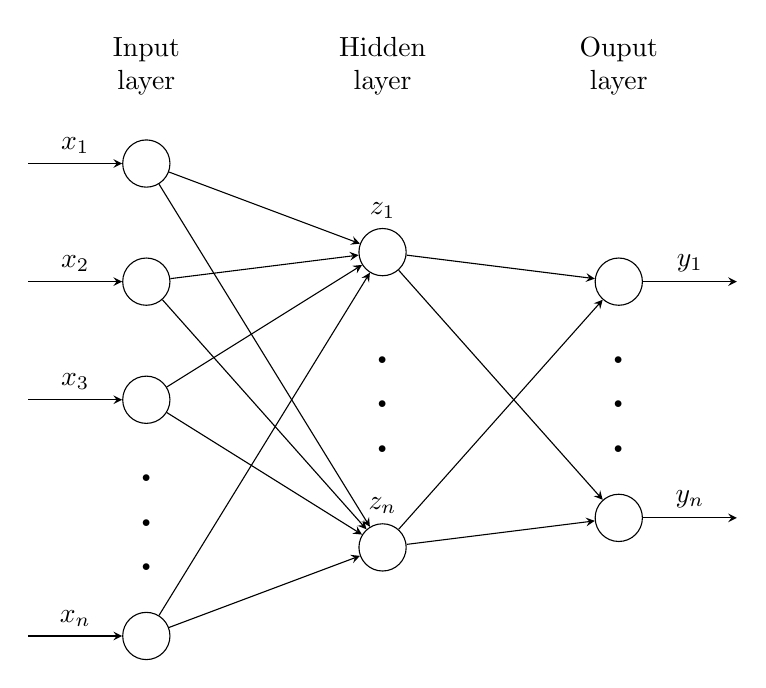
\begin{tikzpicture}[x=1.5cm, y=1.5cm, >=stealth]
        % Inputs nodes
        \foreach \m/\l [count=\y] in {1,2,3,missing,4}
          \node [every neuron/.try, neuron \m/.try] (input-\m) at (0,2.5-\y) {};
        % Hidden nodes
        \foreach \m [count=\y] in {1,missing,2}
          \node [every neuron/.try, neuron \m/.try ] (hidden-\m) at (2,2-\y*1.25) {};
        % Outputs nodes
        \foreach \m [count=\y] in {1,missing,2}
          \node [every neuron/.try, neuron \m/.try ] (output-\m) at (4,1.5-\y) {};
        % Names on inputs
        \foreach \l [count=\i] in {1,2,3,n}
          \draw [<-] (input-\i) -- ++(-1,0)
            node [above, midway] {$x_\l$};
        % Names on hidden
        \foreach \l [count=\i] in {1,n}
          \node [above] at (hidden-\i.north) {$z_\l$};
        % Names on outputs
        \foreach \l [count=\i] in {1,n}
          \draw [->] (output-\i) -- ++(1,0)
            node [above, midway] {$y_\l$};
        % Inputs -> Hidden
        \foreach \i in {1,...,4}
          \foreach \j in {1,...,2}
            \draw [->] (input-\i) -- (hidden-\j);
        % Hidden -> Outputs
        \foreach \i in {1,...,2}
          \foreach \j in {1,...,2}
            \draw [->] (hidden-\i) -- (output-\j);
        % Layer names
        \foreach \l [count=\x from 0] in {Input, Hidden, Ouput}
          \node [align=center, above] at (\x*2,2) {\l \\ layer};
    \end{tikzpicture}
    \caption{Caption}
    \label{fig:my_label}
\end{figure}